\documentclass[conference]{IEEEtran}
\IEEEoverridecommandlockouts
% The preceding line is only needed to identify funding in the first footnote. If that is unneeded, please comment it out.
\usepackage{cite}
\usepackage{amsmath,amssymb,amsfonts}
\usepackage{algorithmic}
\usepackage{graphicx}
\usepackage{textcomp}
\usepackage{xcolor}
\usepackage{hyperref}
\usepackage{svg}
\svgpath{{./figure/}}

\usepackage{listings}
\usepackage{color}

\definecolor{dkgreen}{rgb}{0,0.6,0}
\definecolor{gray}{rgb}{0.5,0.5,0.5}
\definecolor{mauve}{rgb}{0.58,0,0.82}

\lstset{frame=tb,
  language=Python,
  aboveskip=3mm,
  belowskip=3mm,
  showstringspaces=false,
  columns=flexible,
  basicstyle={\small\ttfamily},
  numbers=none,
  numberstyle=\tiny\color{gray},
  keywordstyle=\color{blue},
  commentstyle=\color{dkgreen},
  stringstyle=\color{mauve},
  breaklines=true,
  breakatwhitespace=true,
  tabsize=3
}

\def\BibTeX{{\rm B\kern-.05em{\sc i\kern-.025em b}\kern-.08em
    T\kern-.1667em\lower.7ex\hbox{E}\kern-.125emX}}
\usepackage[backend=biber]{biblatex}
\addbibresource{references.bib}


\begin{document}

\title{Distributed Systems and Cloud Computing \\ 
B3 Project: Election Distributed Algorithms}

\author{\IEEEauthorblockN{Mattia Di Battista (0304938)}
\IEEEauthorblockA{\textit{Università degli studi di Roma "Tor vergata"}\\
Rome, Italy \\
mattia.dibattista@alumni.uniroma2.eu}
}

\maketitle

\begin{abstract}
Election distributed algorithms are a specific implementation of consensus distributed algorithms in which the aim is to find a leader. In this work, Chang and Roberts, and Bully algorithms are implemented with several services. Furthermore, we deploy the whole decentralized network on Docker containers and execute it on an AWS EC2 instance.
\end{abstract}

\begin{IEEEkeywords}
Ring-based algorithm, Bully algorithm, TCP, Docker, AWS EC2, Ansible
\end{IEEEkeywords}

\section{Introduction}
This work aims to implement two election distributed algorithms, make a decentralized network of nodes using \textbf{Docker} containers and execute the whole application on an \textbf{AWS EC2} instance. 
In the following, we describe the services used by the algorithms, the implementation of the algorithms (i.e., \textbf{Chang and Roberts} and \textbf{Bully} algorithms), the whole architecture where to perform them, and three tests used to demonstrate the operation.

\section{Services}

\subsection{Register Service}\label{register}

The \textbf{register service} provides knowledge of the entire network to all nodes belonging to it. Moreover, it generates a unique random ID for each member of the topology (see \ref{fig:register}). 

The register node listens by default on the \textbf{TCP} port \textit{1234} (it can be changed from \textit{SDCC/sdcc/local_config.json}). The listening window is kept open for a \textit{SOCKET\_TIMEOUT} period (defined in \textit{SDCC/sdcc/register/src/constants.py}) after which a node receives the member's network list. 

Initially, every node has an ID equal to \textit{DEFAULT\_ID} (by default set to \textit{-1}). Instead, the register is identified by value \textit{0}. After the register phase, a unique ID to each node is associated.

A node generates multiple sockets for whole its activity. During the register phase, two sockets are created: the first used to communicate with the register node and the second one used later to listen to eventual packets from other nodes. IP address, port, and ID of this latest must be sent before its use to make known to other nodes that information.

\subsection{Heartbeat}

The \textbf{heartbeat service} allows detaching crashes by the coordinator nodes. 

The service is kept active using a thread that sends heartbeat messages to the leader through a dedicated \textbf{TCP} socket (different from the two defined in \ref{register}). After the heartbeat message the thread waits for a while (i.e., \textit{TOTAL\_DELAY} period defined in \textit{SDCC/sdcc/node/src/constants.py}). If the timeout occurs a crash is found out and consequently a new election is started. Only the ACK message indicates a running coordinator.   

\begin{figure}[htbp]
  \centering
  \includesvg[inkscapelatex=false, width = 245pt]{heartbeat.svg}
  \caption{Heartbeat service invoked by two nodes.}
\end{figure}
Heartbeat messages are sent periodically based on the \textit{HEARTBEAT\_TIME} constant. 
If the received message has a different type from HEARTBEAT or the sender is not the current coordinator the packet is ignored and the thread keeps listening for the remaining time. 

\subsection{Verbose}

The \textbf{verbose flag} shows all messages exchanged (i.e., received, sent) throughout the node lifetime\footnote{Also register node implements this service.} (see \ref{fig:verbose}). 
To activate the verbose flag is necessary to pass the \textit{-v} parameter from the command line (see \ref{how}). 

The main info shown are:
\begin{itemize}
    \item Timestamp
    \item Node info (i.e., IP address, port number, ID)
    \item Receiver/Sender info (i.e., IP address, port number, ID)
    \item Message content
\end{itemize}

The \textbf{Logging} library is used to define the message syntax.

\begin{lstlisting}
def set_logging() -> logging:
    logging.basicConfig(
        level=logging.DEBUG,
        format="[%(levelname)s] %(asctime)s\n%(message)s",
        datefmt='%b-%d-%y %I:%M:%S'
    )
    return logging
\end{lstlisting}\caption{Method to instantiate a logging object.}

\subsection{Delay}\label{delay}

To stress more the system, the \textbf{delay method} is introduced in \textit{SDCC/sdcc/node/src/helper.py}. It generates a period waited by the sender to forward the current packet. This may cause the receiver timeout to expire.
\begin{lstlisting}
def delay(flag: bool, ub: int):
    if flag:
        delay = randint(0, floor(ub*1.5))
        time.sleep(delay)
\end{lstlisting}
It is activated by default when tests are performed (see. \ref{sec:tests}), but is also configured by the command line through the \textit{-d} flag.

\section{Algorithm Implementation}

What follows does not describe how the algorithms work, but only how particular aspects are implemented (reference at \cite{coulouris2005distributed}).

The implementation consists of the abstract class \footnote{Defined in \textit{SDCC/sdcc/node/src/Algorithm.py}} and election distributed algorithms classes that extend the first one. 

\begin{figure}[htbp]
  \centering
  \includesvg[inkscapelatex=false, width = 245pt]{class.svg}
  \caption{Logic implementation of the classes.}
\end{figure}

Six types of messages can be exchanged between nodes:

\begin{lstlisting}
class Type(Enum):
    ELECTION = 0
    END = 1
    ANSWER = 2
    HEARTBEAT = 3
    REGISTER = 4
    ACK = 5
\end{lstlisting}
ANSWER type is used only by the \textbf{Bully algorithm}, whereas REGISTER is sent during register phase.

Both algorithms begin with run the listening thread after which they start an election. Only after completing these two phases, the heartbeat can start. 
\begin{lstlisting}
def __init__(self, ...):
        ...
        self.lock = Lock()
        
        thread = Thread(target=self.listening)
        thread.daemon = True
        thread.start()

        self.start_election()
        Algorithm.heartbeat(self)
\end{lstlisting}
Many data are accessed simultaneously from multiple threads, thus a \textbf{lock} is defined to manage shared resources.
\begin{lstlisting}
self.lock.acquire()
if self.participant or (self.coordinator in [self.id, DEFAULT_ID]):
    self.lock.release()
    continue
\end{lstlisting}\caption{Example of \textbf{lock} management in heartbeat method.}

\subsection{Chang and Roberts Algorithm}\label{ring}

The algorithm is suitable for a collection of processes arranged in a logical ring. Each process has a
communication channel to the next one in the ring. All messages
are sent clockwise around the ring. The ID's node is used to define the \textbf{ring network}: the next node is the one with the greatest ID then current and the lowest among others.

\begin{figure}[htbp]
  \centering
  \includesvg[inkscapelatex=false, width = 245pt]{ring_1.svg}
  \caption{Election started by node with \textit{id=23} in Ring topology.}
\end{figure}

When a leader crash occurs or the node's timer associated with a heartbeat message elapses, the leader is removed from the nodes list, therefore remaining nodes can not interact with it even if it is still active.  

\subsection{Bully Algorithm}

With different respect to the \textbf{Ring-based algorithm}, the \textbf{Bully algorithm} assumes that each process knows which processes have higher identifiers and that it can communicate with all such processes. That information is sent by the register node (as described in \ref{register}) 

\begin{figure}[htbp]
  \centering
  \includesvg[inkscapelatex=false, width = 245pt]{bully_1.svg}
  \caption{Election started by node with \textit{id=23} using \textbf{Bully algorithm}.}
\end{figure}

\subsubsection{Scenarios}

Unlike in the \ref{ring}, for the \textbf{Bully algorithm}, the current leader is not removed from the nodes list during leader crash or timeout scenarios.

The considered cases when the leader is executing are:  

\begin{enumerate}
    \item If the leader delays sending the ACK packet, other nodes start a new election that will produce the next coordinator also if the previous one is running\footnote{In the next election it will be elected again.}.
    \item If the leader is stopped\footnote{Using $Ctrl\ +\ z$ combination.} a new election will start. In the meanwhile all messages sent to the sleeping node are queued, so when it wakes up\footnote{Using \textit{fg} command.} will receive those messages and begin the leader again.
\end{enumerate}

\section{Tests}\label{sec:tests}

The following tests are performed:

\begin{enumerate}
    \item \textit{Test A}: a generic node fails
    \item \textit{Test B}: the coordinator fails
    \item \textit{Test C}: both generic and coordinator nodes fail
\end{enumerate}

To interrupt a specific node \href{https://pypi.org/project/psutil/}{\textbf{psutil}} library is used. It kills a process that is listening on a certain \textbf{TCP} port\footnote{It requires root privileges (see \ref{how}).}. That mechanism exploits the sorted list of nodes send by the register. E.g., the fact that the coordinator node occupies the last position in the list is used in \textit{Test B}. 

\begin{lstlisting}
def kill_node(self, port: int):
        for proc in process_iter():
            for conns in proc.connections(kind='inet'):
                if conns.laddr.port == port:
                    proc.send_signal(signal.SIGINT)
\end{lstlisting}

The network is keep running for a while before the test and after the interruption to show its activity.

Test execution is interactive (see \ref{fig:tests}) means that the user chooses which test executes sees logging information on the terminal and sets which algorithm has to be performed.

As described in \ref{delay} to stress more the application, the delay option is active.

\section{Deployment}

The network is deployed on an \textbf{AWS EC2} instance where every node runs on a \textbf{Docker} container. 
\href{https://docs.docker.com/compose/}{\textbf{Docker Compose}} is used to automate the container's creation\footnote{See \textit{SDCC/sdcc/docker-compose.yml},  \textit{SDCC/sdcc/node/Dockerfile} and \textit{SDCC/sdcc/register/Dockerfile}.}. 

By default, \textbf{Docker Compose} creates a network where containers can communicate with each other, so that is used. 

\begin{figure}[htbp]\label{fig:arch}
  \centering
  \includesvg[inkscapelatex=false, width = 245pt]{arch.svg}
  \caption{Deployment using \textbf{AWS EC2} instance and \textbf{Docker} containers.}
\end{figure}

To automate the deployment procedure \href{https://www.ansible.com/}{\textbf{Ansible}} is used to install \textbf{Docker} and to forward the code application on an \textbf{EC2} instance. See \ref{fig:aws}.

\section{How To Use}\label{how}

The application can be run in two different ways:

\begin{enumerate}
    \item Local execution without \textbf{Docker} containers
    \item Remote execution on \textbf{AWS EC2} instance using \textbf{Docker} containers \footnote{That execution requires an \textbf{AWS} account.}(as shown in \ref{fig:arch})
\end{enumerate}

The complete list of commands is available \href{https://github.com/matt-merman/SDCC#running}{here}.

\section{Running Examples}

\begin{figure}[htb]\label{fig:register}
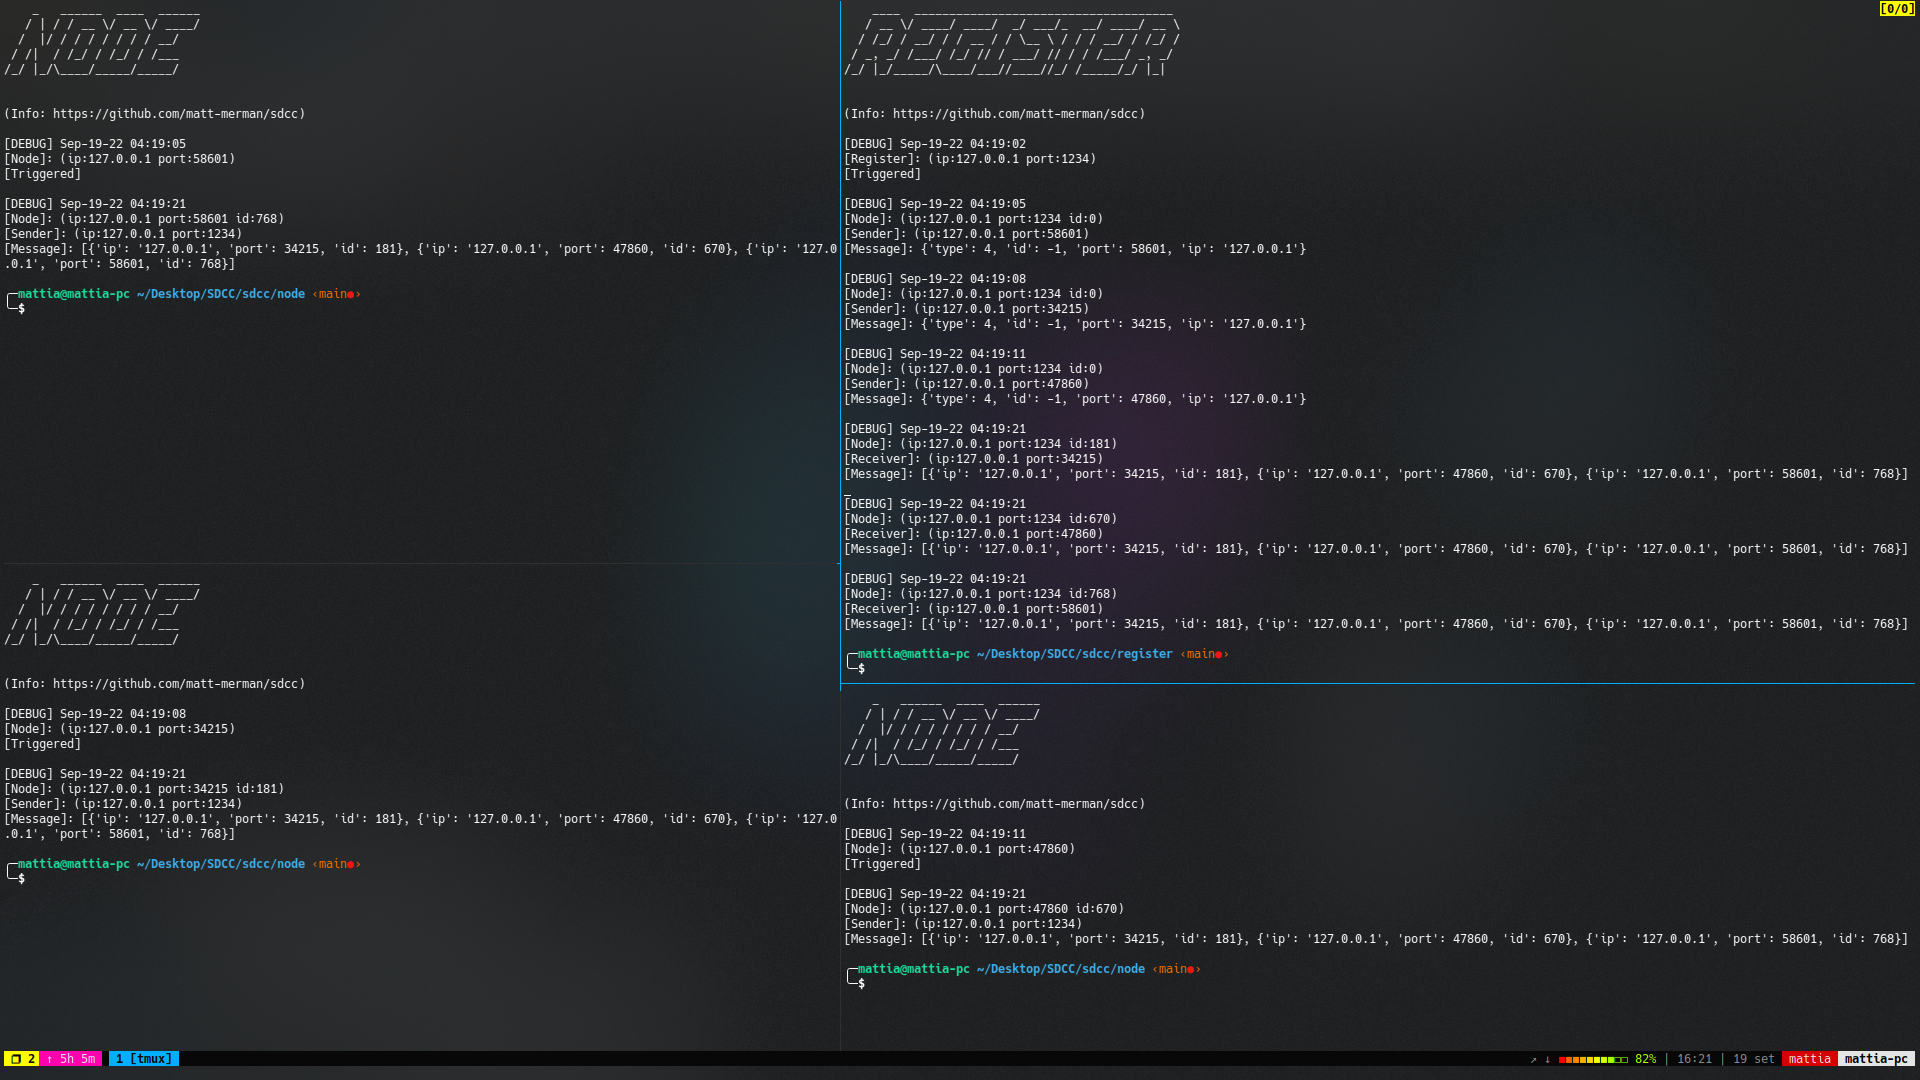
\includegraphics[width=\linewidth]{figure/register_terminal.png}
\caption{Register phase from three generic nodes and register node.}
\end{figure}

\begin{figure}[htb]\label{fig:verbose}
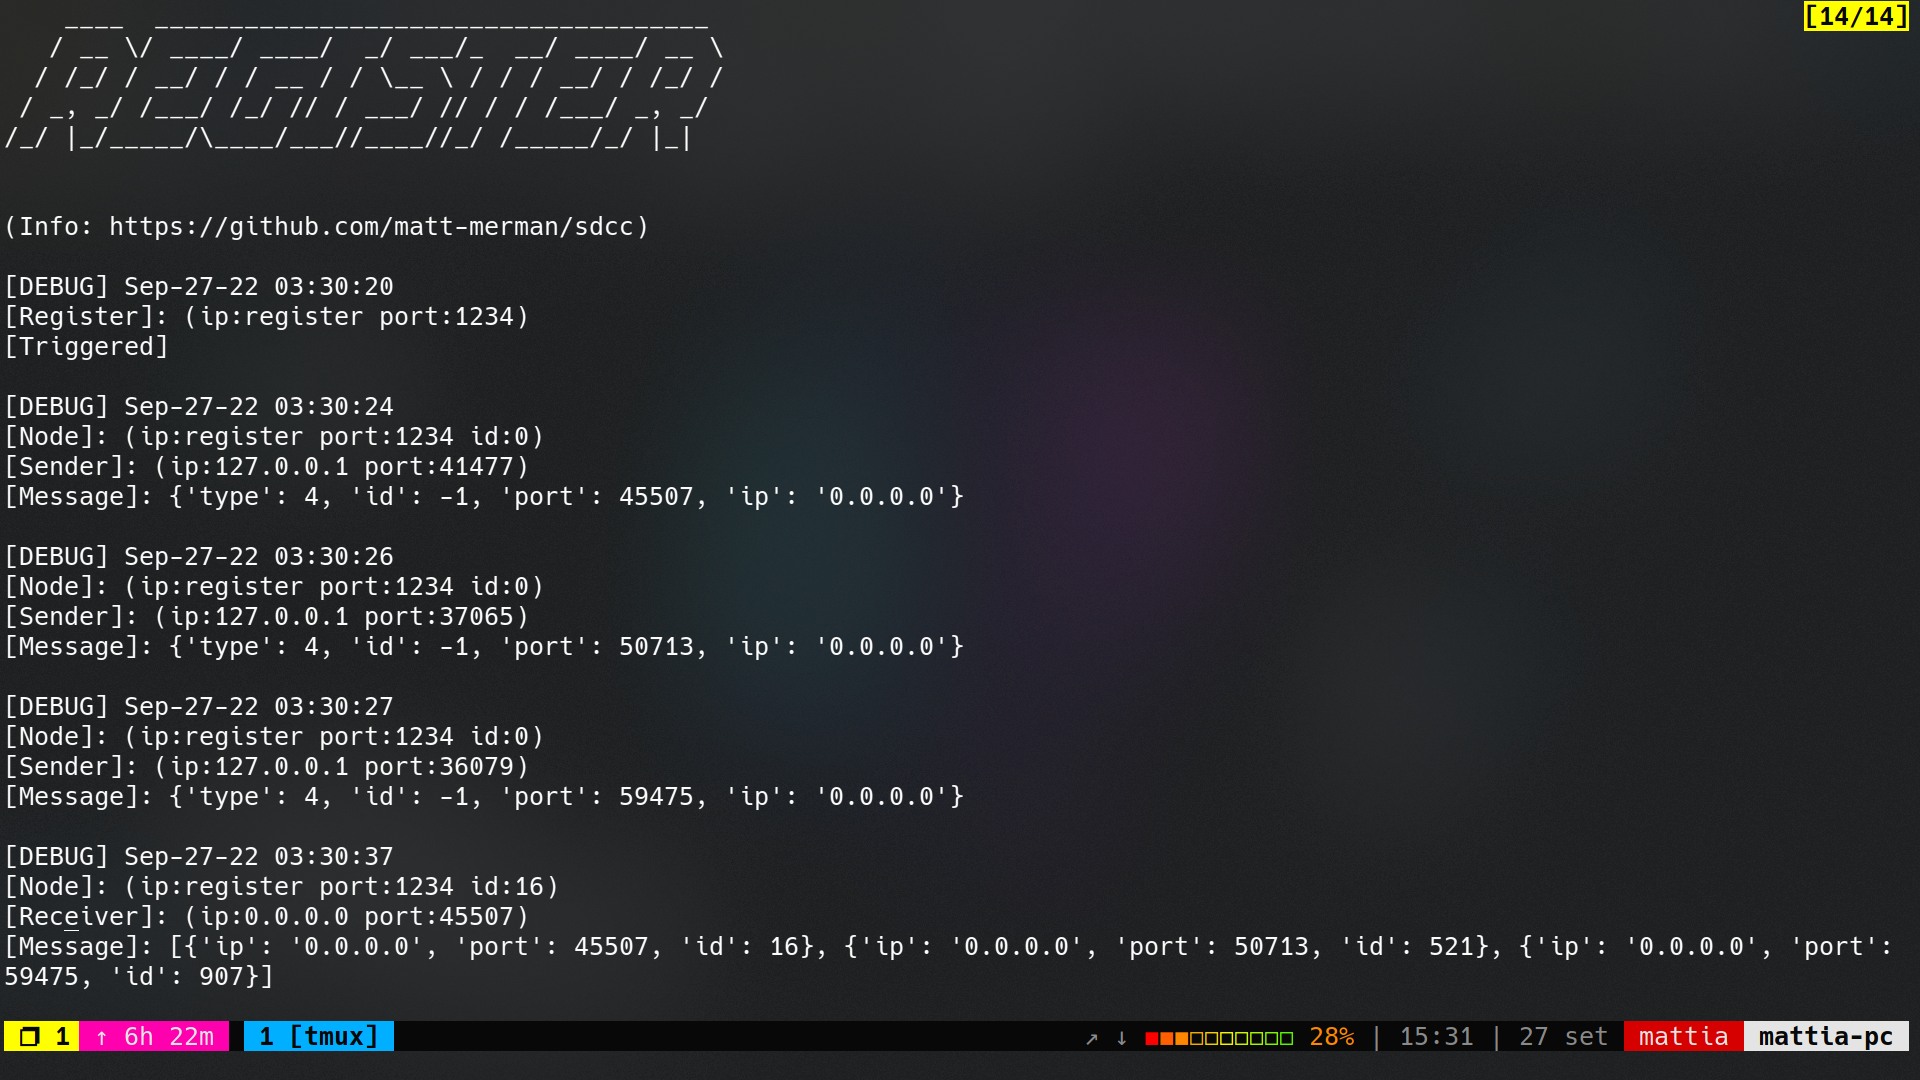
\includegraphics[width=\linewidth]{figure/verbose.png}
\caption{Example of the message showed by register node.}
\end{figure}

\begin{figure}[htb]\label{fig:tests}
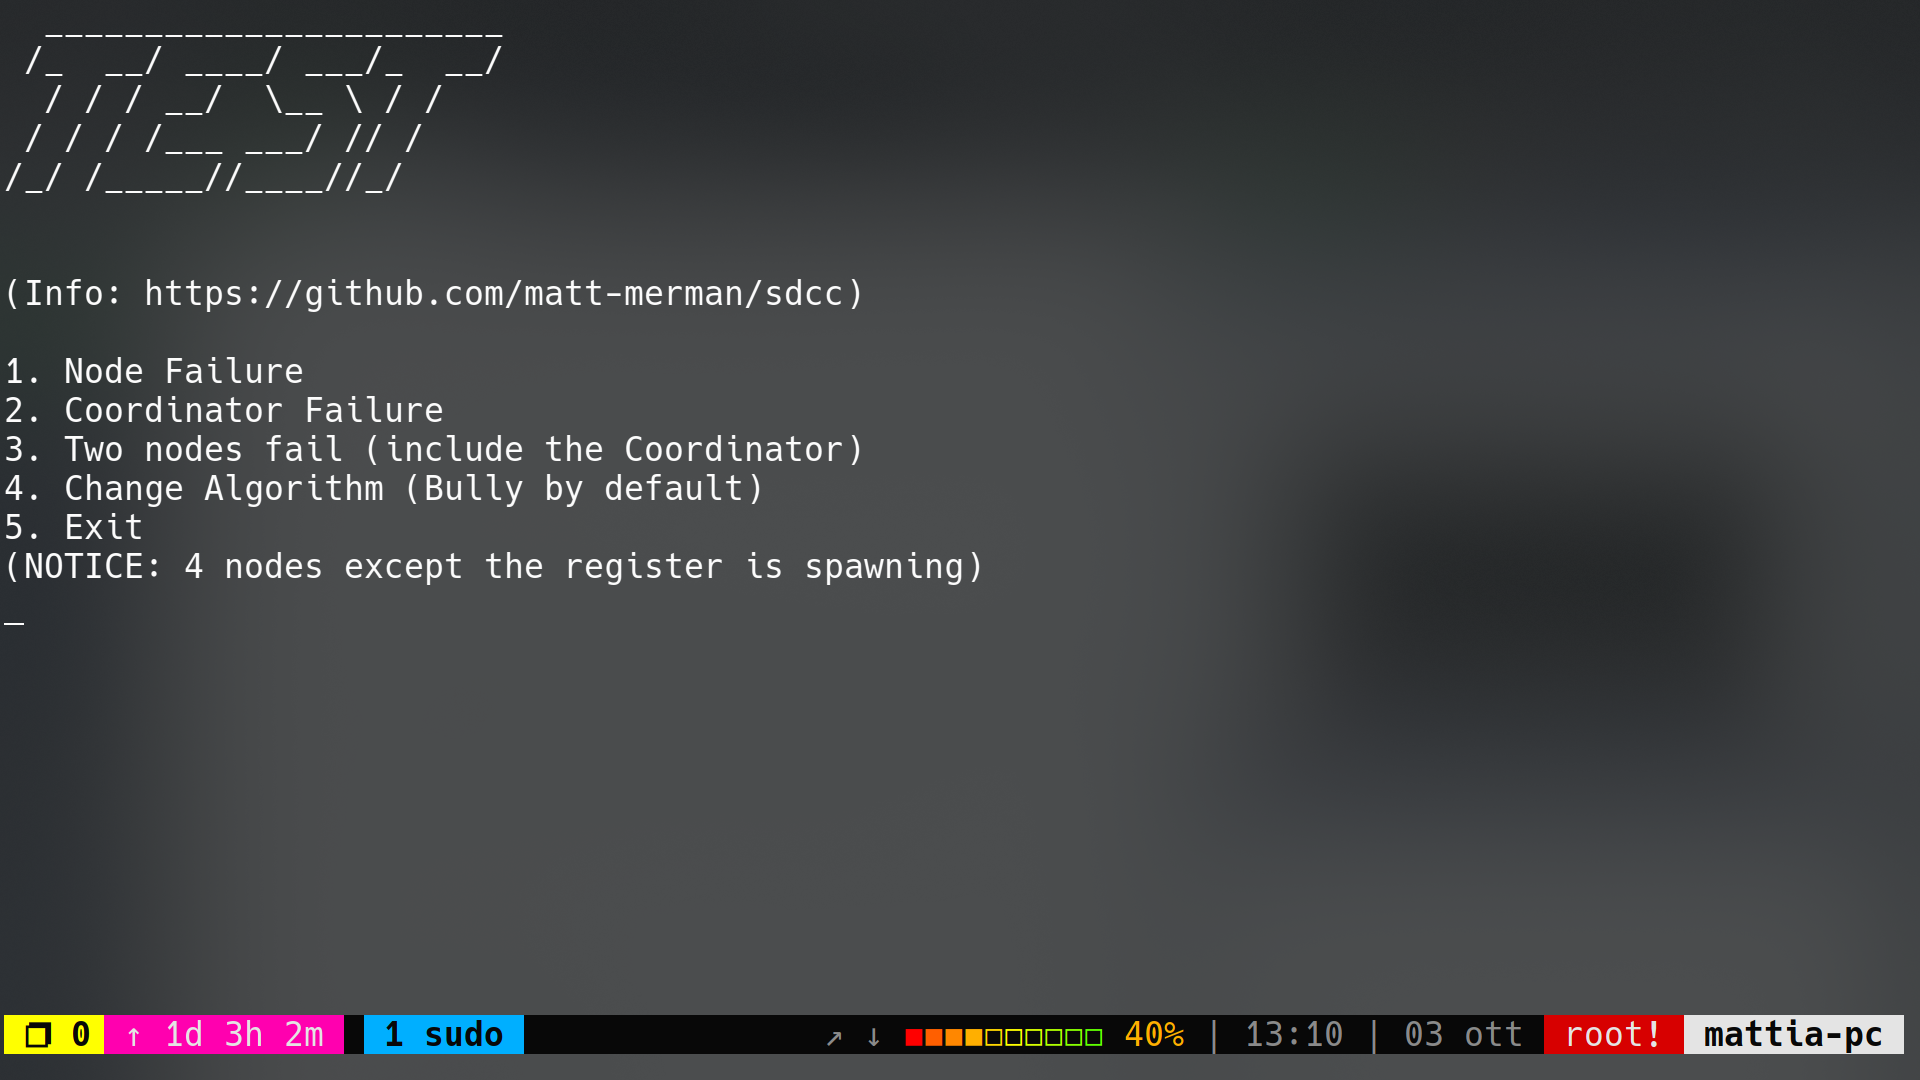
\includegraphics[width=\linewidth]{figure/tests.png}
\caption{User interface to tests execution}
\end{figure}

\begin{figure}[htb]\label{fig:aws}
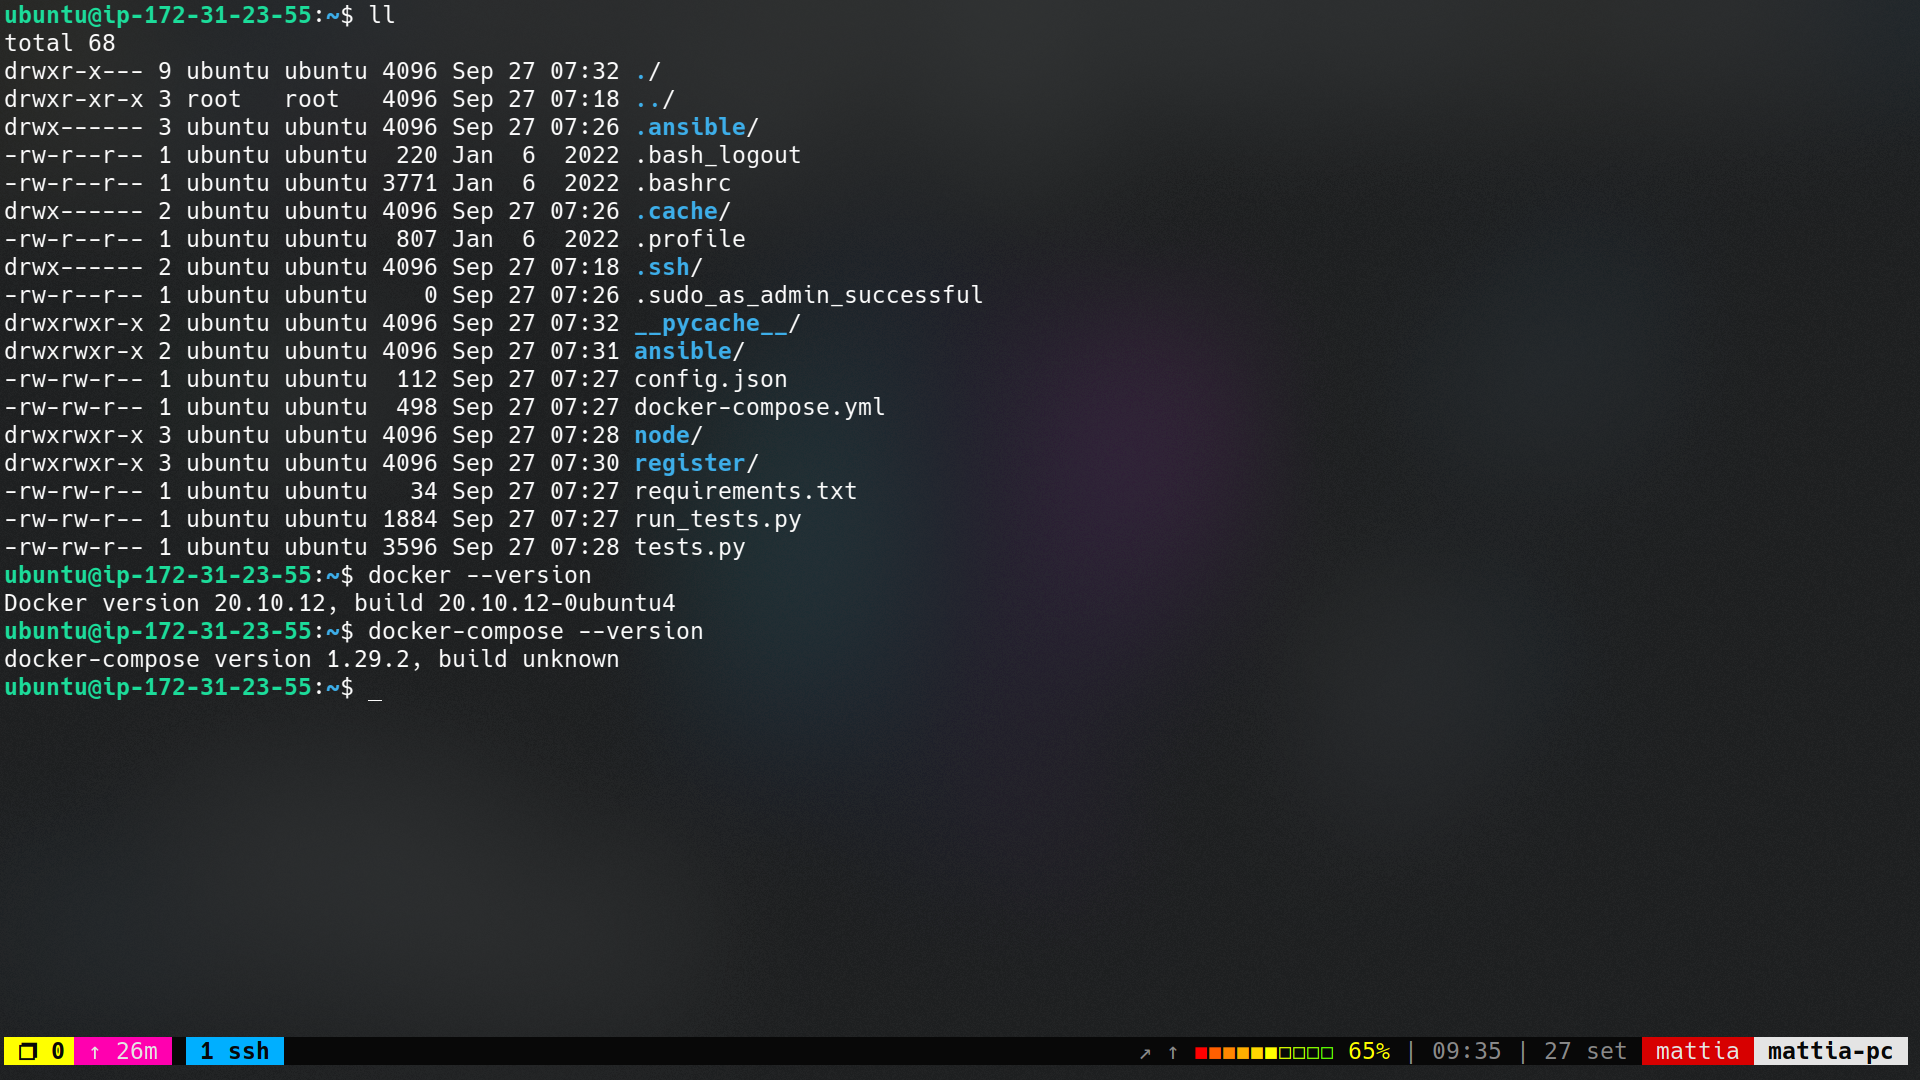
\includegraphics[width=\linewidth]{figure/aws_demo.png}
\caption{\textbf{Docker}, \textbf{Docker Compose} and application code info on an \textbf{AWS EC2} instance.}
\end{figure}

\printbibliography

\end{document}